\chapter{Linear Second-Order Equations}
\chapter*{Lecture 12}
\begin{recall}{}{}
\begin{itemize}
\item Mathematical models:
\begin{itemize}
\item Electric circuits
\item Compartmental analysis (flow in/out of compartment)
\item Heating and cooling
\item Newtonian Mechanics (object falling)
\end{itemize}
\end{itemize}
\end{recall}



\section{Introduction}
\subsection{LRC circuit}
\begin{minipage}{0.65\textwidth}
Starting with an example:\\
Suppose we have a LRC circuit (follows Kirchhoff's law)
\begin{equation}
\boxed{RI(t) + L\frac{dI(t)}{dt}+\frac{1}{C}\int I(t) dt=E}
\label{eq:secondO}
\end{equation}
\end{minipage}
\begin{minipage}{0.28\textwidth}
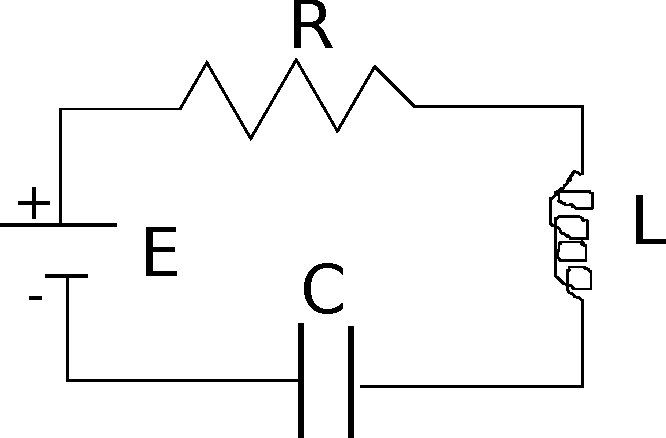
\includegraphics[width=\textwidth]{figs/LRCcircuit.pdf} 
\end{minipage}
\vspace{0.5cm}
The equation is an \textbf{integro-differential} equation.  
How can we convert this equation into a differential equation? Two methods come to mind:
\begin{itemize}
\item Take the derivative of the equation with respect to $t$:
\begin{equation*}
R\frac{dI}{dt}+L\frac{d^2I}{dt^2}+\frac{1}{C}I(t)=\frac{dE}{dt}
\end{equation*}
which corresponds to the ODE for current.
\item Recall $Q=\int I\,dt$ or $I=\frac{dQ}{dt}$. If we sub into \eqref{eq:secondO}, we obtain:
\begin{equation*}
R\frac{dQ}{dt}+L\frac{d^2Q}{dt^2}+\frac{1}{C}Q=E
\end{equation*}
which is the equation for charge.\\
\textbf{Note that both ODEs are second-order linear equations}\\
We recall:
\begin{itemize}
\item \textbf{linear:} coefficients of the derivatives of 'I' or 'Q' are constant or functions of independent variable alone
\item  \textbf{second-order:} highest-order of the derivative 
\end{itemize}
 

\end{itemize}



\subsection{Mass-damper system}
Newton's second law ($F=ma$) is a second-order differential equation when we consider that the acceleration is ($a=d^2 y/dx^2$). \\

We now consider a mass-spring oscillator system
as shown in the figure.
\begin{figure}
\centering
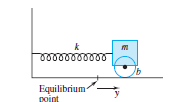
\includegraphics[width=0.4\textwidth]{figs/MassSpring.png}
\caption{Mass-spring system} 
\end{figure}
If the spring is unstretched and the mass is at rest, the system is in equilibrium. As the spring is stretched from its equilibrium state, Hooke's law suggests that the force of the spring is directly proportional to its displacement, $y$, thus:
\begin{equation*}
F_{spring}=-ky
\end{equation*}
where $k$ is known as the spring stiffness.\\
\begin{figure}
\centering
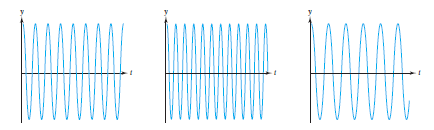
\includegraphics[width=0.8\textwidth]{figs/springStiff.png}
\caption{Spring stiffness} 
\end{figure}
All mass-spring oscillators have some level of friction in the system that acts to dampen the oscillations. Typically friction is acurately modelled by assuming that the frictional force is proportional to the instantaneous velocity:
\begin{equation*}
F_{friction}=-b\frac{dy}{dt}
\end{equation*}
where $b$ is the damping coefficient (generally positive).\\
External forces may also be applied to the mass-spring-damper system such that the general governing equation is:

\begin{equation*}
my'' =- ky -b\frac{dy}{dt}+F_{ext}
\end{equation*}
or
\begin{equation}
\boxed{my'' +b\frac{dy}{dt}+ ky =F_{ext}}
\end{equation}


[Show example from Python]

\subsection{General classification of second-order ODEs}
General form of a 2nd order, linear ODE is:
\begin{equation*}
\boxed{a_2(x)\frac{dy}{dx} +a_1(x)\frac{dy}{dx}+ a_0(x)y =F(x)}
\end{equation*}
Standard form:
\begin{equation*}
\boxed{\frac{d^2y}{dx^2} +p(x)\frac{dy}{dx}+ q(x) y=f(x)}
\end{equation*}
where $f(x)$ is often refered to as the "forcing function".



\subsubsection{Classification of linead second-order ODEs}
Second-order ODEs are distinguished by:
\begin{itemize}
\item coefficients of the dependent variable (and its derivative)
\begin{itemize}
\item constant coefficient 
\item variable coefficient
\end{itemize}
\item forcing function on the right hand side:
\begin{itemize}
\item homogeneous ($f(x)=0$)
\item inhomogeneous (otherwise)
\end{itemize}
\end{itemize}

\begin{center}
\noindent\rule{4cm}{0.4pt}
\end{center}

\begin{exmp}{Current in a LR circuit:}\\
Classify the following LRC circuit for a constant imposed voltage:
\begin{equation}
R\frac{dI}{dt}+L\frac{d^2I}{dt^2}+\frac{1}{C}I(t)=\frac{dE}{dt}
\end{equation}
We have a constant coefficient and homogeneous equation (as $\frac{dE}{dt}$ is null since $E$ is constant)
\end{exmp}
\begin{center}
\noindent\rule{4cm}{0.4pt}
\end{center}

%
%
%\section{Solution superposition in homogeneous ODEs}
%Let's suppose you have the following (homogeneous) second-order ODE:
%\begin{equation*}
%\frac{d^2 y}{dx^2}=y
%\end{equation*}
%By looking at the equation we can identify the solutions:
%\begin{itemize}
%\item $y=e^x$ since $\frac{d^2 y}{dx^2}= \frac{d^2 e^x}{dx^2}=e^x$
%\item $y=e^{-x}$ since $\frac{d^2 y}{dx^2}= \frac{d^2 e^{-x}}{dx^2}=e^{-x}$
%\end{itemize} 
%what about this solution?
%\begin{equation*}
%y=c_1 e^{x}+ c_2e^{-x}
%\end{equation*}
%For the sake of the example, we suppose that $c_1=3$ and $c_2=2/5$.
%
%\begin{eqnarray*}
%y''-y = (c_1 e^{x}+ c_2e^{-x})''- (c_1 e^{x}+ c_2e^{-x})=\\
%3 e^{x} + 2/5e^{-x} - (3 e^{x}+ 2/5e^{-x})=0
%\end{eqnarray*}
%
%
%This last solution tells us that there are an infinite number of solutions to this ODE (since the constants may take any values).
%\\
%\textbf{For a homogeneous linear equation, we can always obtain new solutions from known solutions by multiplication by constant or by addition.} \\
%
%This is called a \textbf{linear combination} of solutions. We will refer to this as the  \textbf{superposition principle} or the \textbf{linearity principle}.\\
%
%NOTE: this theory does not hold for nonhomogeneous linear equations or non-linear equations!!!
%\begin{center}
%\noindent\rule{4cm}{0.4pt}
%\end{center}
%
%\begin{exmp}{Linearity priciple of a nonhomogeneous DE:}\\
%Suppose the following ODE:
%\begin{equation*}
%y''+y=1
%\end{equation*}
%(this is a nonhomogeneous, linear, 2nd-order ODE).
%Show that the priciple of linearity does NOT hold.\\
%\textbf{Solution:}
%The solutions of this ODE are $y_1=1+cos(x)$ and $y_2=1+sin(x)$. Is the linear superposition of these two also a solution to the ODE?\\
%$y=c_1 y_1 + c_2 y_2 = c_1(1+cos(x))+c_2(1+sin(x))$:
%(suppose $c_1=c_2=1$ for simplicity)
%\begin{eqnarray*}
%(2+cos(x)+sin(x))''+(2+cos(x)+sin(x))-1=0\\
%-cos(x)-sin(x)+(2+cos(x)+sin(x))-1\neq 0\\
%\end{eqnarray*}
%The linear combination of the two solutions is NOT a solution to the ODE. (because the solution is nonhomogeneous)
%\end{exmp}
%\begin{center}
%\noindent\rule{4cm}{0.4pt}
%\end{center}
%
%It is also important to remember that in order to apply the superposition, the solutions must be linearly independent from one another!
%
%\begin{center}
%\noindent\rule{4cm}{0.4pt}
%\end{center}
%\begin{exmp}{Linear independence:}\\
%Coming back to the first example:
%\begin{equation*}
%\frac{d^2 y}{dx^2}=y
%\end{equation*}
%Is the following superposed solution also a solution to the ODE?
%\begin{equation*}
%y=2 e^x+ 4 e^x
%\end{equation*}
%This solution does not satisfy the ODE!
%[Prove!]
%\end{exmp}
%\begin{center}
%\noindent\rule{4cm}{0.4pt}
%\end{center}